\documentclass[11pt,a4paper]{article}

\usepackage{fontspec}
\usepackage{xeCJK}
\setmainfont{Liberation Serif}
\setsansfont{Liberation Sans}
\setmonofont{DejaVu Sans Mono}
\setCJKmainfont{Noto Serif CJK SC}
\setCJKsansfont{Noto Sans CJK SC}
\setCJKmonofont{Noto Sans Mono CJK SC}

\usepackage[margin=1.8cm]{geometry}
\usepackage{amsmath,amssymb,mathtools,bm}
\usepackage{booktabs,longtable,tabularx,array,multirow}
\usepackage{graphicx}
\usepackage{float}
\usepackage{xcolor}
\usepackage{xurl}
\usepackage{enumitem}
\usepackage{caption}
\usepackage{hyperref}

\definecolor{linkblue}{RGB}{30,85,145}
\definecolor{lightblue}{RGB}{235,244,252}
\definecolor{lightgray}{RGB}{245,245,245}
\definecolor{darkgreen}{RGB}{25,110,75}
\hypersetup{
  colorlinks=true,
  linkcolor=linkblue,
  urlcolor=linkblue,
  citecolor=linkblue
}
\captionsetup{font=small,labelfont=bf}
\setlist{nosep,leftmargin=2em}
\setlength{\parindent}{2em}
\setlength{\parskip}{0.35em}
\setlength{\emergencystretch}{3em}
\renewcommand{\arraystretch}{1.18}
\renewcommand{\abstractname}{摘要}
\renewcommand{\contentsname}{目录}
\renewcommand{\figurename}{图}
\renewcommand{\tablename}{表}
% Liberation Serif 没有 small caps；方法缩写统一用无衬线大写。
\renewcommand{\textsc}[1]{\textsf{\MakeUppercase{#1}}}

\newcommand{\R}{\mathbb{R}}
\newcommand{\dd}{\,\mathrm{d}}
\newcommand{\E}{\mathbb{E}}
\newcommand{\piB}{\pi_\beta}
\newcommand{\KL}{D_{\mathrm{KL}}}
\newcommand{\ESS}{\mathrm{ESS}}
\newcommand{\LSC}{\textsc{lsc-cp}}
\newcommand{\PT}{\textsc{pt}}
\newcommand{\CP}{\textsc{cp}}
\newcommand{\RA}{\textsc{ra}}
\newcommand{\MA}{\textsc{ma}}
\newcolumntype{L}[1]{>{\raggedright\arraybackslash}p{#1}}
\newcolumntype{C}[1]{>{\centering\arraybackslash}p{#1}}
\newcolumntype{Y}{>{\raggedright\arraybackslash}X}

\title{\textbf{Lévy Score-Corrected Compound-Poisson\\
平衡采样数值实验中文总结}}
\author{讨论与协作稿}
\date{2026年7月}

\begin{document}
\maketitle

\begin{abstract}
本文档面向组内讨论与协作，集中解释 Lévy score-corrected
compound-Poisson（LSC-CP）平衡采样实验的系统设置、评价指标、自由能反应坐标、
终态分布误差、时间序列有效样本量、能量偏差、计算成本和数值稳定性。四个测试体系
分别是一维双阱、二维四十模高斯混合、十维深度平衡 Müller--Brown 模型以及二十四维
耦合 $\phi^4$ 模型。结果显示，稳定化 LSC-CP 在所测试步长和有限时域内显著促进了
跨盆地探索，并改善了盆地占比和低维自由能面的恢复；与此同时，MoG40 的部分全局
分布指标尚未达到参考底噪，实际有限步链还存在可统计分辨的能量偏差。本文档用于
解释和讨论，不替代英文 manuscript-ready experiment section。
\end{abstract}

\tableofcontents
\clearpage

\section{一页式结论}

\begin{table}[H]
\centering
\small
\begin{tabularx}{\textwidth}{L{2.4cm}YYY}
\toprule
体系 & LSC-CP 的主要结果 & 与主要基线的比较 & 最重要的限定 \\
\midrule
双阱 &
盆地 TV 为 $0.0036$，达到有限样本参考底噪；worst-basin ESS 为 $1648$。 &
PT 的 $W_2$ 和 FES RMSE 更小；LSC 的 basin ESS 高于 PT。 &
LSC 的能量均值偏差为 $+0.194$，明显大于 MCSE。 \\
MoG40 &
盆地 TV 为 $0.064$，达到参考带；盆地 KL 为 $0.012$，显著优于 PT 和 raw CP。 &
LSC 的盆地占比恢复最好；PT 的 post-settling basin ESS 更高。 &
$W_2=2.83$ 和 MMD $=0.0482$ 仍高于参考带，说明完整几何分布尚有残差。 \\
MB 10D &
$W_2=0.047$、TV $=0.014$，与 PT 一样达到参考底噪；worst-basin ESS 为 $1952$。 &
LSC 与 PT 基本打平：LSC 的 $W_2$ 略小，PT 的 TV、FES RMSE 和吞吐率略优。 &
LSC 能量偏差 $+0.039$ 虽数值不大，但约为 $27$ 个 MCSE。 \\
耦合 $\phi^4$ &
$W_2=0.100$、TV $=0.022$、FES RMSE $=0.151$，终态误差表中整体最好。 &
LSC 的终态盆地恢复优于 PT；PT 的 worst-basin ESS/s 明显更高。 &
参考 SNIS 与长 PT 之间已有 basin TV $0.042$ 的差异；LSC 能量偏差为 $+0.251$。 \\
\bottomrule
\end{tabularx}
\caption{四个体系的核心结果和正确解读。}
\end{table}

\noindent
最稳妥的总括是：
\begin{quote}
在所测试的四个模型体系、步长和有限时间范围内，稳定化 LSC-CP 实现显著促进了
跨盆地探索，并改善了盆地占比与低维自由能面的恢复；但完整分布误差和观测量依赖
的有限步偏差仍然存在。因此，结果支持“增强平衡采样”，不支持“实际有限步链精确
无偏”。
\end{quote}

\section{研究问题、系统和实验规模}

所有实验的目标都是 Boltzmann 分布
\begin{equation}
 \pi_\beta(x)=Z_\beta^{-1}\exp[-\beta V(x)].
\end{equation}
研究问题不是重建物理反应动力学，而是在强亚稳性下更快地恢复平衡分布、盆地质量和
热力学观测量。

\begin{table}[H]
\centering
\small
\begin{tabularx}{\textwidth}{L{2.2cm}C{0.8cm}C{0.9cm}C{1.3cm}C{1.0cm}C{1.2cm}C{1.0cm}Y}
\toprule
体系 & $d$ & $\beta$ & 粒子数 & $T$ & $\Delta t$ & seeds & 主要采样难点 \\
\midrule
双阱 & 1 & 8 & 16000 & 100 & 0.005 & 24 &
两个等深势阱之间存在 $\beta\Delta V=8$ 的势垒，检验两态平衡和跨阱通信。 \\
MoG40 & 2 & 8 & 2500 & 100 & 0.010 & 24 &
四十个远距离等权高斯模态；跳跃设计不使用模态位置。 \\
深度平衡 MB & 10 & 24 & 2000 & 200 & 0.005 & 16 &
二维 Müller--Brown 有效景观嵌入十维；$A\leftrightarrow B$ 势垒约为 $11.1\,k_{\rm B}T$。 \\
耦合 $\phi^4$ & 24 & 8 & 1000 & 100 & 0.002 & 16 &
十二个二维格点形成四个相位，跃迁要求多体集体移动。 \\
\bottomrule
\end{tabularx}
\caption{实验系统和主要配置。所有体系的跳跃率均为 $\lambda=1$。}
\end{table}

\subsection{跳跃几何}

\begin{table}[H]
\centering
\small
\begin{tabularx}{\textwidth}{L{2.2cm}C{1.0cm}L{4.1cm}Y}
\toprule
体系 & 原子数 $A$ & 跳跃 bank & 设计含义 \\
\midrule
双阱 & 2 & 位于 $\pm2$、径向半宽 $0.2$ 的对称壳层 &
将一个势阱附近的样本直接送到另一个势阱附近。 \\
MoG40 & 连续环形 law & 半径均匀分布于 $[4,15]$，方向在圆周上均匀 &
只使用典型模态间距，不使用四十个模态中心的位置。 \\
MB & 4 & $A\to B$、$B\to A$、$B\to C$、$C\to B$ &
只保留中继图，无直接 $A\leftrightarrow C$ 原子，要求通过中间盆地 $B$。 \\
$\phi^4$ & 8 & 四相方形边上的八个有向集体原子 &
删除穿过场零点高能区域的两组对角跃迁；对角转换通过两个边跳中继完成。 \\
\bottomrule
\end{tabularx}
\caption{四个体系的跳跃设计。}
\end{table}

\section{方法和基线}

\begin{longtable}{L{2.5cm}L{4.0cm}L{7.8cm}}
\toprule
方法 & 含义 & 在本文中的作用和注意事项 \\
\midrule
\endfirsthead
\toprule
方法 & 含义 & 在本文中的作用和注意事项 \\
\midrule
\endhead
\textsc{ula} &
Unadjusted Langevin algorithm &
局部过阻尼 Langevin 离散。单盆地内部混合可以很快，但跨越高势垒很慢，且有限步长会产生离散误差。 \\
\textsc{mala} &
Metropolis-adjusted Langevin algorithm &
用接受/拒绝校正 Langevin proposal；目标分布正确，但仍然依赖局部 proposal，跨盆地困难。 \\
\textsc{baoab} &
欠阻尼 Langevin BAOAB 积分器 &
带动量的局部基线。在本实验时域内仍无法覆盖所有盆地。 \\
\textsc{fla} &
$\alpha$-stable Lévy flight analogue &
重尾长跳跃对照。它的目标不变分布不是 $\pi_\beta$，因此不能把较小的某个终态误差解释为正确平衡采样。 \\
\textsc{pt} &
Parallel tempering &
通过多个温度副本改善跨势垒通信。所有效率比较计入完整副本成本。 \\
raw \textsc{cp} &
只有 compound-Poisson jump，没有 Lévy-score 校正 &
用于检验 score 校正是否必要。其不变分布不是 $\pi_\beta$，所以是 stationarity-defect 消融，而不是公平的平衡采样效率基线。 \\
\textsc{lsc-cp} &
Lévy-score-corrected compound-Poisson &
在局部 Langevin 漂移上同时加入非局部跳跃和与该 jump law 匹配的 Lévy-score 漂移。 \\
\textsc{lsc-cp-ra} &
单原子随机估计器 &
每粒子每步只抽取一个随机位移，并在 score 与 jump 中复用；成本低但估计方差较大。 \\
\textsc{lsc-cp-ma} &
配对多原子随机估计器 &
每粒子每步为每个原子族各抽取一个位移，并在 score 与逐原子 Poisson jump 中复用同一 bank；用于 MB 和 $\phi^4$。 \\
\bottomrule
\end{longtable}

\section{指标应该怎样阅读}

\begin{longtable}{L{2.8cm}L{8.4cm}C{2.3cm}}
\toprule
指标 & 含义 & 好坏方向 \\
\midrule
\endfirsthead
\toprule
指标 & 含义 & 好坏方向 \\
\midrule
\endhead
$W_2$ &
样本分布与参考分布之间的 Wasserstein-2 距离。双阱中为一维精确值；高维体系在声明的低维 metric space 中计算 sliced $W_2$。 &
越小越好 \\
Basin TV &
盆地占比总变差：
$\mathrm{TV}_{\rm basin}=\frac12\sum_k|\widehat p_k-p_k^\star|$。只衡量宏观盆地质量，不衡量盆地内部形状。 &
越小越好 \\
Basin KL &
$\KL(p^\star\Vert\widetilde p)$，使用 Jeffreys 伪计数。这个方向会强烈惩罚遗漏目标盆地。 &
越小越好 \\
FES RMSE &
消除自由能任意加法常数后，样本自由能面与参考自由能面的加权均方根误差，单位为 $k_{\rm B}T$。 &
越小越好 \\
FES outside &
样本的集体变量落在预先冻结的参考 FES 网格之外的质量。网格内部 RMSE 必须与该值一起阅读。 &
越小越好 \\
MMD &
由核函数定义的全局分布差异。MoG40 中它揭示了 basin population 正确但全局几何仍不完整的情况。 &
越小越好 \\
IAT &
积分自相关时间。时间序列相关越强，IAT 越大。 &
越小越好 \\
ESS &
相关样本等价于多少个独立样本，近似为 $N/\tau_{\rm int}$。 &
越大越好，但需结合偏差 \\
Worst-basin ESS &
对每个盆地指示函数计算 ESS 后取最小值，衡量最难访问盆地的可用统计信息。 &
越大越好 \\
Energy ESS &
只衡量势能时间序列的去相关速度，不等价于全局盆地混合。 &
越大越好，但需结合 bias \\
Signed energy bias &
轨迹平均势能减去目标平均势能。正值表示平均势能偏高，负值表示偏低。 &
绝对值越小越好 \\
MCSE &
Monte Carlo standard error，常用 $s/\sqrt{\ESS}$ 估计。它衡量随机估计误差，不会自动消除离散核的系统偏差。 &
越小越好 \\
Split-$\widehat R$ &
多链一致性诊断。接近 1 表示链间与链内变化更一致；它不能验证目标分布本身正确。 &
越接近 1 越好 \\
ESS/s &
单位墙钟时间产生的有效样本量。只有在准确度和计费范围相当时，才能直接用于排名。 &
越大越好 \\
弱恒等式残差 &
有限测试函数上的生成器级 drift--jump 抵消残差。它不包含 taming、cap、Euler splitting 和 box projection。 &
越小越好 \\
\bottomrule
\end{longtable}

\paragraph{表中括号的含义。}
终态指标采用“跨 seed 均值（标准差）”格式。例如
$0.064\,(0.008)$ 表示均值为 $0.064$、seed 间标准差为 $0.008$。

\section{反应坐标、集体变量和自由能面}

自由能面必须相对于一个声明的集体变量
\begin{equation}
 s=\xi(x)
\end{equation}
来定义。该坐标上的边缘概率密度为
\begin{equation}
 p_\xi(s)=\int \delta\!\left(s-\xi(x)\right)\pi_\beta(x)\dd x,
\end{equation}
对应自由能
\begin{equation}
 F_\xi(s)=-\beta^{-1}\log p_\xi(s)+C.
\end{equation}
本文报告以 $k_{\rm B}T$ 为单位的约化自由能，因此
\begin{equation}
 \frac{F_\xi(s)}{k_{\rm B}T}=-\log p_\xi(s)+C.
\end{equation}

\begin{table}[H]
\centering
\small
\begin{tabularx}{\textwidth}{L{2.3cm}L{4.2cm}C{1.1cm}Y}
\toprule
体系 & FES 使用的 $\xi(x)$ & 维度 & 解释 \\
\midrule
双阱 & $\xi(x)=x$ & 1 &
原始位置坐标，同时也是完整构型坐标。 \\
MoG40 & $\xi(x)=(x_1,x_2)$ & 2 &
完整二维构型坐标，没有额外降维。 \\
MB 10D & $\xi(x)=(z_1,z_2)$ & 2 &
Müller--Brown 势能所在的二维 latent/active coordinates；八个高斯辅助维度被边缘化。 \\
耦合 $\phi^4$ &
$\displaystyle \xi(q)=\bar q=\frac1{12}\sum_{i=1}^{12}q_i$ &
2 &
空间平均序参量，用于区分四个相位；非均匀场涨落被投影掉。 \\
\bottomrule
\end{tabularx}
\caption{自由能分析使用的集体变量。}
\end{table}

在离散网格中，第 $i$ 个单元概率为 $p_i$、单元面积或体积为 $|C_i|$，约化自由能为
\begin{equation}
 A_i=-\log\frac{p_i}{|C_i|}.
\end{equation}
由于自由能只确定到加法常数，FES RMSE 在比较前拟合一个最佳常数。只在参考概率
$p_i^\star\ge 5/N$ 的 supported cells 上计算加权 RMSE；落在冻结网格外的质量单独
报告为 FES outside。

\paragraph{术语限定。}
这些坐标更准确地说是用于平衡分析的集体变量或序参量，并未验证为精确 committor
或物理动力学意义上的最优反应坐标。沿这些坐标得到的自由能不能直接解释为真实反应
路径或反应速率。

\section{有限样本参考底噪 floor}

Floor 不是理论上的严格下界，而是两个相同样本量的独立参考样本相互比较时产生的经验
误差尺度。本文把
\begin{equation}
 \text{floor band 上界}=\text{reference-reference 均值}
 +3\times\text{reference-reference 标准差}
\end{equation}
作为“达到 floor”的判据。进入该带表示当前误差无法与有限样本参考噪声清楚区分，
不表示误差严格为零，也不等价于证明收敛。

\begin{table}[H]
\centering
\small
\begin{tabularx}{\textwidth}{L{2.3cm}C{3.0cm}C{3.0cm}Y}
\toprule
体系 & $W_2$ floor；上界 & TV floor；上界 & LSC-CP 解读 \\
\midrule
双阱 &
$0.061\pm0.033$；$0.160$ &
$0.0032\pm0.0017$；$0.0083$ &
$W_2=0.111$、TV $=0.0036$，两者均进入参考带。 \\
MoG40 &
$1.31\pm0.28$；$2.15$ &
$0.051\pm0.006$；$0.069$ &
TV $=0.064$ 进入参考带；$W_2=2.83$ 未进入。 \\
MB &
$0.050\pm0.020$；$0.110$ &
$0.011\pm0.007$；$0.032$ &
$W_2=0.047$、TV $=0.014$，两者均进入参考带。 \\
$\phi^4$ &
$0.130\pm0.035$；$0.235$ &
$0.024\pm0.010$；$0.054$ &
$W_2=0.100$、TV $=0.022$，两者均进入参考带。 \\
\bottomrule
\end{tabularx}
\caption{有限样本 floor 及 LSC-CP 是否进入参考带。}
\end{table}

\section{终态平衡恢复：完整数值}

本节所有误差指标均为越小越好。FLA 和 raw CP 不以 $\pi_\beta$ 为不变分布，因此
只能作为非目标对照或 score 消融，不能与目标正确的采样器进行无条件的效率排名。

\subsection{双阱}

\begin{table}[H]
\centering
\footnotesize
\setlength{\tabcolsep}{4.2pt}
\begin{tabular}{lccccc}
\toprule
方法 & $W_2$ & Basin TV & FES RMSE & Basin KL & Outside \\
\midrule
\textsc{ula} & $1.26\,(.003)$ & $.471\,(.001)$ & $1.77\,(.02)$ & $1.09\,(.02)$ & $0$ \\
\textsc{mala} & $1.26\,(.003)$ & $.473\,(.001)$ & $1.79\,(.02)$ & $1.12\,(.02)$ & $0$ \\
\textsc{baoab} & $1.29\,(.002)$ & $.488\,(.001)$ & $2.23\,(.04)$ & $1.54\,(.04)$ & $0$ \\
\textsc{fla} & $.096\,(.018)$ & $.0033\,(.003)$ & $.302\,(.008)$ & $3.4{\times}10^{-5}$ & $.003$ \\
\textsc{pt} & $.064\,(.032)$ & $.0033\,(.002)$ & $.050\,(.009)$ & $3.2{\times}10^{-5}$ & $0$ \\
raw \textsc{cp} & $.176\,(.013)$ & $.0036\,(.003)$ & $.157\,(.006)$ & $4.2{\times}10^{-5}$ & $.029$ \\
\textbf{\textsc{lsc-cp}} & $.111\,(.017)$ & $.0036\,(.003)$ & $.168\,(.009)$ & $4.4{\times}10^{-5}$ & $.005$ \\
\textsc{lsc-cp-ra} & $.131\,(.017)$ & $.0031\,(.003)$ & $.180\,(.010)$ & $3.2{\times}10^{-5}$ & $.008$ \\
\bottomrule
\end{tabular}
\caption{双阱终态指标，格式为均值（标准差）。}
\end{table}

\paragraph{解释。}
三种局部方法的盆地 TV 约为 $0.47$--$0.49$，说明仍然严重偏向初始阱。PT 的全局
$W_2$ 和 FES RMSE 最小。LSC-CP 与 RA 都恢复了左右盆地质量并进入 TV floor。
raw CP 的 basin TV 看似很小，但它的目标分布不正确，且有 $2.9\%$ 的质量位于参考
FES 网格外。

\subsection{MoG40}

\begin{table}[H]
\centering
\footnotesize
\setlength{\tabcolsep}{4.2pt}
\begin{tabular}{lccccc}
\toprule
方法 & $W_2$ & Basin TV & FES RMSE & Basin KL & Outside \\
\midrule
\textsc{ula} & $26.1\,(.02)$ & $.916\,(.003)$ & $1.81\,(.01)$ & $4.20\,(.02)$ & $0$ \\
\textsc{mala} & $26.1\,(.03)$ & $.917\,(.003)$ & $1.81\,(.01)$ & $4.21\,(.01)$ & $0$ \\
\textsc{baoab} & $26.2\,(.03)$ & $.930\,(.005)$ & $1.77\,(.01)$ & $4.24\,(.02)$ & $0$ \\
\textsc{fla} & $15.2\,(.21)$ & $.436\,(.007)$ & $1.37\,(.06)$ & $.743\,(.05)$ & $.001$ \\
\textsc{pt} & $6.54\,(.34)$ & $.141\,(.007)$ & $.350\,(.02)$ & $.055\,(.005)$ & $0$ \\
raw \textsc{cp} & $9.98\,(.19)$ & $.286\,(.009)$ & $.680\,(.04)$ & $.267\,(.013)$ & $.254$ \\
\textbf{\textsc{lsc-cp}} & $2.83\,(.34)$ & $.064\,(.008)$ & $.190\,(.02)$ & $.012\,(.003)$ & $.001$ \\
\textsc{lsc-cp-ra} & $2.65\,(.26)$ & $.103\,(.009)$ & $.280\,(.02)$ & $.036\,(.006)$ & $.005$ \\
\bottomrule
\end{tabular}
\caption{MoG40 终态指标，格式为均值（标准差）。}
\end{table}

\paragraph{解释。}
LSC-CP 的盆地 TV、KL 和 FES RMSE 在目标方法中最好，TV 已进入参考 floor。
RA 的 $W_2=2.65$ 略小于确定性/半解析 LSC 的 $2.83$，但其 TV、KL、FES RMSE
和 outside 均更差。因此 RA 只能作为估计器敏感性检查，不能称为与确定性 score
数值等价。最重要的负结果是：LSC 的 $W_2=2.83$ 高于 floor 上界 $2.15$，
MMD $=0.0482$ 也高于参考带上界约 $0.0317$。这说明四十个模态的质量已经接近正确，
但完整全局几何分布仍有残差。raw CP 有 $25.4\%$ 的质量落在参考 FES 网格外，而
LSC 只有 $0.1\%$。

\subsection{Müller--Brown 10D}

\begin{table}[H]
\centering
\footnotesize
\setlength{\tabcolsep}{4.2pt}
\begin{tabular}{lccccc}
\toprule
方法 & $W_2$ & Basin TV & FES RMSE & Basin KL & Outside \\
\midrule
\textsc{ula} & $.409\,(.003)$ & $.307\,(.002)$ & $2.27\,(.23)$ & $1.17\,(.14)$ & $0$ \\
\textsc{mala} & $.411\,(.003)$ & $.308\,(.001)$ & $2.32\,(.18)$ & $1.22\,(.16)$ & $0$ \\
\textsc{baoab} & $.415\,(.003)$ & $.309\,(.001)$ & $2.50\,(.17)$ & $1.52\,(.21)$ & $0$ \\
\textsc{fla} & $.179\,(.006)$ & $.119\,(.008)$ & $.941\,(.04)$ & $.048\,(.007)$ & $.039$ \\
\textsc{pt} & $.056\,(.021)$ & $.013\,(.008)$ & $.132\,(.02)$ & $5.7{\times}10^{-4}$ & $0$ \\
raw \textsc{cp} & $.353\,(.008)$ & $.135\,(.006)$ & $.267\,(.02)$ & $.047\,(.005)$ & $.172$ \\
\textbf{\textsc{lsc-cp-ma}} & $.047\,(.009)$ & $.014\,(.006)$ & $.136\,(.010)$ & $5.8{\times}10^{-4}$ & $.006$ \\
\bottomrule
\end{tabular}
\caption{深度平衡 MB 10D 终态指标，格式为均值（标准差）。}
\end{table}

\paragraph{解释。}
PT 和 LSC-CP-MA 的 $W_2$、TV、FES RMSE 和 KL 基本打平，并且 $W_2$ 与 TV
都进入参考底噪。LSC 的 $W_2$ 略小；PT 的 TV、FES RMSE 和 KL 略小。raw CP
有 $17.2\%$ 的样本质量位于参考网格外，LSC 为 $0.6\%$。

\subsection{耦合 \texorpdfstring{$\phi^4$}{phi4} 24D}

\begin{table}[H]
\centering
\footnotesize
\setlength{\tabcolsep}{4.2pt}
\begin{tabular}{lccccc}
\toprule
方法 & $W_2$ & Basin TV & FES RMSE & Basin KL & Outside \\
\midrule
\textsc{ula} & $1.22\,(.004)$ & $.671\,(.003)$ & $2.59\,(.09)$ & $3.07\,(.31)$ & $0$ \\
\textsc{mala} & $1.22\,(.004)$ & $.673\,(.002)$ & $2.63\,(.05)$ & $3.13\,(.17)$ & $0$ \\
\textsc{baoab} & $1.22\,(.006)$ & $.673\,(.002)$ & $2.64\,(.05)$ & $3.14\,(.22)$ & $0$ \\
\textsc{fla} & $.194\,(.032)$ & $.060\,(.013)$ & $.220\,(.03)$ & $.011\,(.004)$ & $10^{-4}$ \\
\textsc{pt} & $.364\,(.028)$ & $.119\,(.015)$ & $.315\,(.04)$ & $.039\,(.008)$ & $0$ \\
raw \textsc{cp} & $.410\,(.021)$ & $.077\,(.016)$ & $.482\,(.05)$ & $.017\,(.006)$ & $.209$ \\
\textbf{\textsc{lsc-cp-ma}} & $.100\,(.028)$ & $.022\,(.011)$ & $.151\,(.03)$ & $.0015\,(.001)$ & $.003$ \\
\bottomrule
\end{tabular}
\caption{耦合 $\phi^4$ 24D 终态指标，格式为均值（标准差）。}
\end{table}

\paragraph{解释。}
LSC-CP-MA 在该表的五个终态指标上均最好，并且 $W_2$ 与 TV 均进入参考底噪。
raw CP 的网格外质量为 $20.9\%$，LSC 为 $0.3\%$。FLA 的若干数字看似有竞争力，
但它并不以 $\pi_\beta$ 为不变分布。$\phi^4$ 的 SNIS 参考与独立长 PT 参考之间已有
basin TV $=0.042$ 的差异，因此小于这一尺度的盆地优劣具有参考敏感性。

\subsection{时间方向上的松弛}

\begin{figure}[H]
\centering
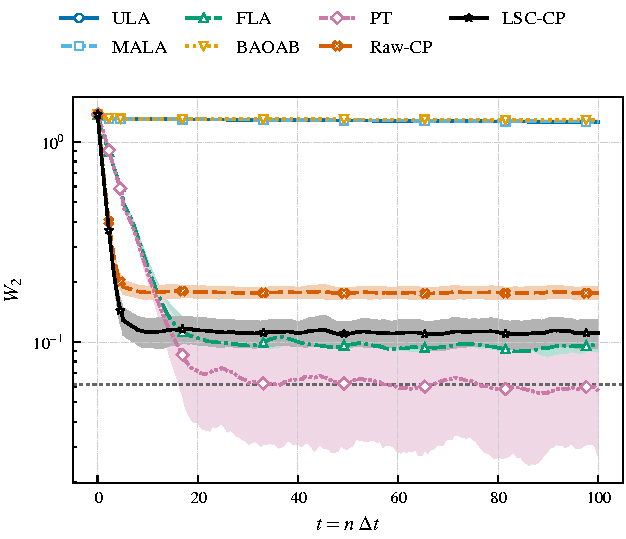
\includegraphics[width=0.48\textwidth]{figs/double_well_W2_t.pdf}
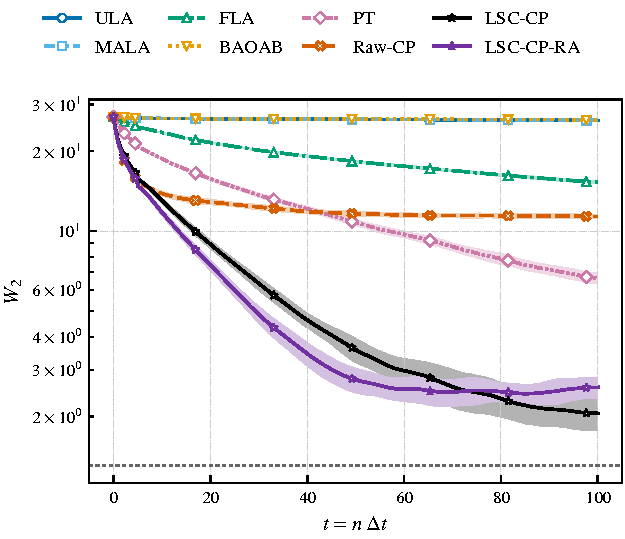
\includegraphics[width=0.48\textwidth]{figs/mog40_W2_t.pdf}\\[3pt]
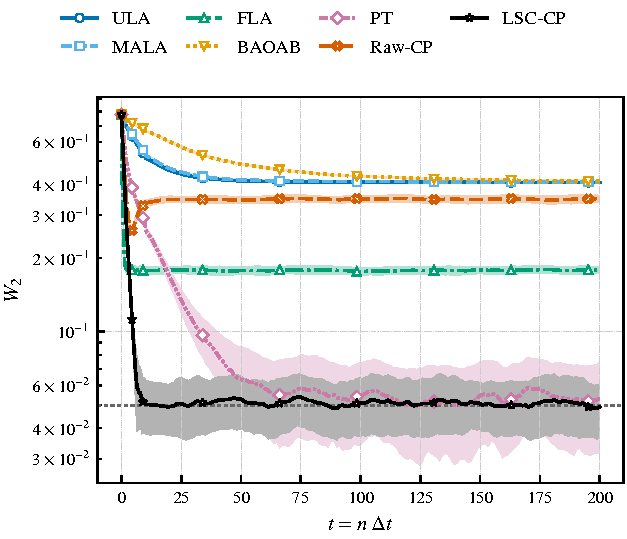
\includegraphics[width=0.48\textwidth]{figs/mb3well_10d_W2_t.pdf}
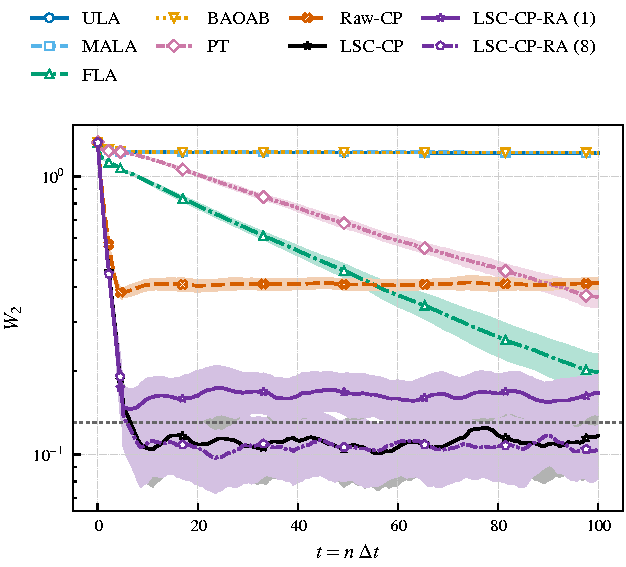
\includegraphics[width=0.48\textwidth]{figs/coupled_phi4_W2_t.pdf}
\caption{从共同局域初始分布出发，$W_2$ 随算法时间的变化。上排：双阱、MoG40；
下排：MB 10D、耦合 $\phi^4$。这些曲线显示非局部方法能够降低全局分布误差，
而局部方法在给定时域内仍强烈亚稳。}
\end{figure}

\section{Post-settling 时间序列、ESS 和偏差}

终态 ensemble 指标衡量时刻 $T$ 的分布误差，不直接给出时间平均的精度。时间序列
实验使用 $4$ 个 seed、每个 seed $8$ 条链、每条链 $1000$ 个等间隔记录，总计
$32000$ 个 post-settling 样本。链从参考分布初始化，先演化一个 settling horizon，
再记录一个 horizon。raw CP 和 FLA 因目标不变分布不是 $\pi_\beta$，未纳入该效率表。

\subsection{Worst-basin ESS}

\begin{table}[H]
\centering
\small
\begin{tabular}{lrrrr}
\toprule
方法 & 双阱 & MoG40 & MB & $\phi^4$ \\
\midrule
\textsc{ula} & 0 & 0 & 0 & 0 \\
\textsc{mala} & 0 & 0 & 0 & 0 \\
\textsc{baoab} & 0 & 0 & 0 & 0 \\
\textsc{pt} & 1211 & 572 & 2336 & 2567 \\
\textbf{\textsc{lsc-cp}} & 1648 & 229 & 1952 & 1150 \\
\textsc{lsc-cp-ra} & 1809 & 59 & --- & --- \\
\bottomrule
\end{tabular}
\caption{Worst-basin ESS，总记录量为 $32000$。越高表示最难采样盆地的占比时间序列
包含越多近似独立信息。}
\end{table}

局部方法的 worst-basin ESS 全为零，说明至少有一个盆地指示函数恒定或没有被有效
访问。这不等于完全没有 label change：MoG40 中 ULA/MALA/BAOAB 分别记录
$222/230/60$ 次变化，MB 中为 $209/194/43$ 次，但这些变化不足以覆盖全部盆地并
形成可用的最慢盆地统计量。LSC 在四个体系中均获得非零 worst-basin ESS。双阱中
LSC 高于 PT；MoG40、MB 和 $\phi^4$ 中 PT 更高。

\subsection{Energy ESS 与 signed energy bias}

\begin{table}[H]
\centering
\scriptsize
\setlength{\tabcolsep}{3.2pt}
\resizebox{\textwidth}{!}{
\begin{tabular}{lcccc}
\toprule
方法 & 双阱：ESS / bias & MoG40：ESS / bias & MB：ESS / bias & $\phi^4$：ESS / bias \\
\midrule
\textsc{ula} & $14815 / +0.0003$ & $707 / +0.001$ & $22223 / +0.007$ & $17212 / +0.133$ \\
\textsc{mala} & $14869 / +0.0005$ & $710 / -0.004$ & $21994 / -0.001$ & $15250 / -0.010$ \\
\textsc{baoab} & $3658 / -0.0002$ & $534 / -0.001$ & $5622 / +0.004$ & $2734 / +0.028$ \\
\textsc{pt} & $20494 / -0.001$ & $1340 / +0.0006$ & $25202 / -0.0004$ & $24383 / -0.002$ \\
\textbf{\textsc{lsc-cp}} & $31891 / +0.194$ & $22718 / +0.114$ & $26720 / +0.039$ & $30972 / +0.251$ \\
\textsc{lsc-cp-ra} & $31224 / +0.247$ & $9165 / +0.448$ & --- & --- \\
\bottomrule
\end{tabular}}
\caption{能量 ESS 与带符号能量偏差。ESS 越高只表示能量去相关快；bias 的绝对值
越小才表示能量均值更准确。}
\end{table}

这张表说明 ESS 不能单独使用。LSC 的 energy ESS 很高，但能量均值存在明确正偏。
另一个典型反例是 MB 中 ULA 的 energy ESS 为 $22223$，而 worst-basin ESS 为零：
粒子可以在单个盆地内部快速改变势能，却没有完成全局混合。

\subsection{偏差是否被 Monte Carlo 误差分辨}

\begin{table}[H]
\centering
\small
\begin{tabular}{lrrr}
\toprule
体系 & LSC energy bias & MCSE & $|\mathrm{bias}|/\mathrm{MCSE}$ \\
\midrule
双阱 & $+0.194$ & $0.0194$ & $10.0$ \\
MoG40 & $+0.114$ & $0.00485$ & $23.5$ \\
MB & $+0.039$ & $0.00143$ & $27.3$ \\
$\phi^4$ & $+0.251$ & $0.0141$ & $17.8$ \\
\bottomrule
\end{tabular}
\caption{LSC-CP 能量偏差与 Monte Carlo standard error。}
\end{table}

所有偏差都远大于 MCSE，因此不是普通抽样波动，而是当前样本量能够清楚分辨的系统
偏差。增加轨迹长度会缩小 MCSE，但不会自动消除由有限步长、有限求积、taming、
score cap 或 box projection 造成的离散核偏差。RA 的对应比值约为：双阱 $9.0$，
MoG40 $27.3$。

\subsection{\texorpdfstring{Split-$\widehat R$}{Split-Rhat}}

能量的 split-$\widehat R$ 在表中方法上均小于 $1.11$，但其他盆地和集体变量并非
如此：

\begin{table}[H]
\centering
\small
\begin{tabular}{lr}
\toprule
方法/体系 & 最大 split-$\widehat R$ \\
\midrule
MoG40 LSC-CP & $1.70$ \\
MoG40 LSC-CP-RA & $1.61$ \\
MoG40 PT & $1.28$ \\
$\phi^4$ PT & $1.13$ \\
\bottomrule
\end{tabular}
\caption{部分方法在所有观测量上的最大 split-$\widehat R$。}
\end{table}

这些值表明并非每个盆地或 collective-variable trace 都已达到良好多链一致性。
$\widehat R$ 也不能验证目标分布本身正确：多条链可能一致地采样同一个有偏离散分布。

\subsection{专用 H200 上的 ESS/s}

只有 MB 与 $\phi^4$ 在无并发 GPU 负载下报告每秒效率。

\begin{table}[H]
\centering
\small
\begin{tabular}{llrrl}
\toprule
体系 & 指标 & LSC-CP & PT & 比较 \\
\midrule
MB & Energy ESS/s & $33.03$ & $48.23$ & PT 约为 $1.46\times$ \\
MB & Worst-basin ESS/s & $2.41$ & $4.47$ & PT 约为 $1.85\times$ \\
$\phi^4$ & Energy ESS/s & $50.80$ & $62.17$ & PT 约为 $1.22\times$ \\
$\phi^4$ & Worst-basin ESS/s & $1.89$ & $6.55$ & PT 约为 $3.47\times$ \\
\bottomrule
\end{tabular}
\caption{专用单张 H200 GPU 上的吞吐率。PT 计入全部温度副本成本。}
\end{table}

在这两个体系的墙钟吞吐率上，PT 更高，尤其 $\phi^4$ 的跨盆地吞吐率优势明显。
另一方面，LSC 在报告时点的部分 terminal population 指标更准确。因此应联合阅读
终态误差、时间序列 ESS、观测量偏差和计算成本，不能用单一数字宣布统一赢家。

\section{LSC-CP-MA 的具体操作}

\subsection{核心思想}

对预先定义的 $A$ 个原子族
$\{r_a,w_a,q_a\}_{a=1}^{A}$，LSC-CP-MA 在每个粒子、每个时间步独立刷新一个
多原子随机 bank。对粒子 $i$，
\begin{equation}
 R_{i,a}\sim q_a,\qquad a=1,\ldots,A,
\end{equation}
并定义粒子特异的随机有限测度
\begin{equation}
 \widehat\nu_i(\dd r)
 =\lambda\sum_{a=1}^{A}w_a\delta_{R_{i,a}}(\dd r).
\end{equation}
同一个 realized bank 同时用于计算 Lévy-score 漂移和生成逐原子的 Poisson jump。
不同粒子不共享 realized bank；所有粒子只共享确定性原子中心、权重和壳层宽度。

\subsection{每一步的真实顺序}

\paragraph{1. 抽取随机 bank。}
对每个粒子和每个原子族，
\begin{equation}
 \rho_{i,a}\sim\mathrm{Unif}(-h_a,h_a),\qquad
 R_{i,a}=r_a+\rho_{i,a}\frac{r_a}{\|r_a\|}.
\end{equation}
生产实验的 Gaussian jitter 为零。bank 张量形状为 $(N,A,d)$，抽样函数没有状态
参数，因此 bank 在结构上独立于当前 $X_n$。

\paragraph{2. 抽取逐原子 Poisson 次数。}
\begin{equation}
 N_{i,a}\sim\operatorname{Poisson}(\lambda w_a\Delta t),
 \qquad
 \Delta J_i=\sum_aN_{i,a}R_{i,a}.
\end{equation}
MA 模式不截断 count。若某个 $N_{i,a}>1$，该步内的多次事件复用同一个
$R_{i,a}$。总期望跳跃数仍为
\begin{equation}
 \sum_a\E[N_{i,a}]=\lambda\Delta t.
\end{equation}

\paragraph{3. 用同一个 bank 计算 score。}
对每个原子和 Gauss--Legendre 节点，
\begin{equation}
 I_{i,a}(X_n)
 \approx
 \sum_{p=1}^{q_\theta}\omega_p
 \exp\!\left\{\beta\left[
 V(X_n)-V(X_n-\theta_pR_{i,a})
 \right]\right\},
\end{equation}
然后
\begin{equation}
 S_{\mathcal R_i,\beta}(X_n)
 =
 -\lambda\sum_{a=1}^{A}w_aR_{i,a}I_{i,a}(X_n).
\end{equation}
实现使用 log-sum-exp，并在所有原子完成相对加权之后，对每个粒子的总
log-magnitude 使用 $M_{\max}=600$ 的 cap。这样在 cap 触发时仍保留原子间相对贡献
和合成方向，只改变总幅度。

\paragraph{4. 组成总漂移并进行 tamed Euler 更新。}
\begin{equation}
 b_n=-\nabla V(X_n)+S_{\mathcal R_i,\beta}(X_n),
\end{equation}
\begin{equation}
 X_n^{\rm pre}
 =
 X_n+
 \Delta t\,\frac{b_n}{1+\Delta t\|b_n\|/c}
 +\sqrt{\frac{2\Delta t}{\beta}}\,\xi_n,
 \qquad \xi_n\sim N(0,I).
\end{equation}
MB 和 $\phi^4$ 使用
\begin{equation}
 h=0.1\min_a\|r_a\|,\qquad c=2h.
\end{equation}
因此大漂移极限下，单步漂移位移长度趋于 $c$。

\paragraph{5. 施加 jump 并投影。}
\begin{equation}
 X_{n+1}^{\rm raw}
 =
 X_n^{\rm pre}+\sum_aN_{i,a}R_{i,a},
 \qquad
 X_{n+1}=\operatorname{clip}_{\mathcal B}(X_{n+1}^{\rm raw}).
\end{equation}
即使该步所有 $N_{i,a}=0$，score 漂移仍然作用。score 不是只在 jump 发生时启动
的事后修正。

\subsection{为什么必须配对}

冻结 realized bank 后，score 和 jump 都对应同一个测度
$\widehat\nu_i$。在精确弦积分和连续生成器层面，漂移项和 jump 项可以逐原子满足弱
抵消。再对随机 bank 取平均有
\begin{equation}
 \E[\widehat\nu_i]=\nu.
\end{equation}
如果 score 使用 bank $\mathcal R$，jump 却独立使用另一个 bank $\mathcal R'$，
即使 score 在边缘平均意义下无偏，每一步的条件 drift--jump 测度仍然失配。

\subsection{MA 不等于“每步跳很多次”}

\begin{table}[H]
\centering
\small
\begin{tabular}{lrrrr}
\toprule
体系 & $A$ & $q_\theta$ & 每原子 Poisson 均值 & 每粒子每步 score 能量差数 \\
\midrule
MB & 4 & 8 & $0.00125$ & $4\times8=32$ \\
$\phi^4$ & 8 & 32 & $0.00025$ & $8\times32=256$ \\
\bottomrule
\end{tabular}
\caption{LSC-CP-MA 的 bank 大小、跳跃稀疏度和 score 成本。}
\end{table}

MA 的“multi-atom”表示每一步的 score 对每个原子族都有一个随机代表。真正的
jump 仍然非常稀疏：MB 每粒子每步总期望 jump 数为 $0.005$，$\phi^4$ 为 $0.002$。

\subsection{确定性、RA 与 MA 的关系}

\begin{table}[H]
\centering
\small
\begin{tabularx}{\textwidth}{L{2.4cm}L{4.5cm}C{2.6cm}Y}
\toprule
版本 & 每粒子每步处理的 jump law & score 成本 & 特点 \\
\midrule
确定性 score &
对原子、径向节点和弦节点做确定性求积 &
$Aq_\rho q_\theta$ &
随机估计方差低，但高维计算昂贵。 \\
RA &
从完整 mixture 中只抽一个位移 $R$ &
$q_\theta$ &
最便宜，但在 MoG40 上 basin ESS 和 KL 对随机估计更敏感。 \\
MA &
每个原子族各抽一个 $R_a$，按 $w_a$ 分层加权 &
$Aq_\theta$ &
覆盖全部跳跃类型，方差和成本介于 RA 与完整确定性求积之间。 \\
\bottomrule
\end{tabularx}
\caption{三种 score 实现的比较。配置表中的 $q_\rho$ 不参与 MA 的逐步 realized-bank
score；MA 直接从连续径向壳层抽取 $\rho_{i,a}$。}
\end{table}

\subsection{有限步实现的边界}

配对结构保证的是给定 realized bank 时 score 与 jump 使用同一测度。它不自动证明
实际有限步链精确保持 $\pi_\beta$，因为实现还包含：

\begin{itemize}
 \item 有限 $q_\theta$ 弦积分；
 \item score log-magnitude cap；
 \item Euler drift/diffusion--jump splitting；
 \item 总漂移 taming；
 \item 有限状态盒 projection；
 \item 同一原子单步多次事件复用同一个 realized displacement。
\end{itemize}

因此，MA 应被表述为“消除 score 与 jump 使用不同随机 bank 的额外失配”，而不是
“使稳定化有限步链精确无偏”。

\section{数值稳定性和诊断}

\begin{table}[H]
\centering
\scriptsize
\setlength{\tabcolsep}{3.2pt}
\resizebox{\textwidth}{!}{
\begin{tabular}{lrrrr}
\toprule
诊断量 & 双阱 & MoG40 & MB & $\phi^4$ \\
\midrule
非有限状态数 & $0$ & $0$ & $0$ & $0$ \\
LSC score-cap 比例 & $5.02\times10^{-4}$ & $0$ & $2.85\times10^{-7}$ & $2.09\times10^{-4}$ \\
状态盒投影比例，各方法最大值 &
$8.67\times10^{-5}$ & $3.84\times10^{-4}$ & $3.304\times10^{-3}$ & $8.903\times10^{-4}$ \\
LSC jump 边界接触率 &
$1.69\times10^{-4}$ & $1.05\times10^{-5}$ & $2.18\times10^{-3}$ & $1.60\times10^{-4}$ \\
raw CP jump 边界接触率 &
$3.03\times10^{-4}$ & $2.475\times10^{-2}$ & $6.733\times10^{-2}$ & $4.130\times10^{-3}$ \\
目标方法盆地映射域逃逸 &
$0$ & $0$ & $0$ & $1.0\times10^{-3}$ \\
未截帽弱恒等式残差 &
$1.5\times10^{-7}$ & $3.0\times10^{-8}$ & $5.0\times10^{-7}$ & $2.0\times10^{-7}$ \\
\bottomrule
\end{tabular}}
\caption{数值稳定性诊断。比例通常越低越好。}
\end{table}

\begin{itemize}
 \item 四个体系的 nonfinite count 均为零，说明稳定化成功避免了 NaN/Inf 爆炸。
 \item 正常轨迹上的 score cap 和 box projection 比例较低，但任何非零触发都会改变
 转移核；低频只支持数值稳健性，不证明精确平稳。
 \item 在故意扩展的弱恒等式诊断网格上，双阱和 MB 的 cap 前指数超阈值比例分别为
 $0.402$ 和 $0.374$；这与真实轨迹上的 activation fraction 不是同一个量。
 \item raw CP 在 MoG40 和 MB 上的 jump 边界接触率分别为 $2.475\%$ 和 $6.733\%$，
 因此有限盒显著混杂了 raw-CP 消融，不能把全部差异都归因于缺少 score。
 \item $\phi^4$ 的 basin-map escape $10^{-3}$ 对应一个粒子在一个 checkpoint 越界，
 不是持续的千分之一稳态概率。
 \item 所有弱恒等式残差均低于 $10^{-6}$，但它只检查未截帽、求积定义的生成器级
 drift--jump 抵消。
\end{itemize}

\section{参考分布及其不确定性}

\begin{table}[H]
\centering
\small
\begin{tabularx}{\textwidth}{L{2.3cm}L{5.1cm}Y}
\toprule
体系 & 参考构造 & 需要注意的地方 \\
\midrule
双阱 &
指定有限盒上的 $2\times10^5$ 点稠密网格逆 CDF &
一维参考精度高，但仍以声明的有限盒为定义域。 \\
MoG40 &
直接从已知等权 Gaussian mixture 精确抽样 &
四个体系中最直接的参考。 \\
MB &
$2400^2$ 二维 latent 网格乘以精确高斯辅助坐标 &
FES、盆地质量和低维 metric space 主要由二维 latent 坐标定义。 \\
$\phi^4$ &
四个相位极小点上的 Laplace mixture proposal，加 self-normalized importance weights &
参考是近似的；必须结合权重 ESS 和独立 PT cross-check 阅读。 \\
\bottomrule
\end{tabularx}
\caption{四个体系的参考分布。}
\end{table}

$\phi^4$ 参考使用 $2\times10^5$ 个 proposal，权重 ESS 为 $41182$，即 $20.6\%$，
最大归一化权重为 $3.6\times10^{-3}$。盆地质量、能量矩、集体变量均值和 FES
直接使用 SNIS 权重；只有 $W_2$、MMD 等要求无权样本的指标才使用有限
sampling-importance-resampling。独立长 PT 得到的相位质量与 SNIS 参考之间的
basin TV 为 $0.042$，因此低于这一尺度的 $\phi^4$ 盆地差异具有参考敏感性。

\section{结果支持什么、不支持什么}

\begin{longtable}{L{8.2cm}C{2.1cm}L{4.0cm}}
\toprule
陈述 & 是否支持 & 原因 \\
\midrule
\endfirsthead
\toprule
陈述 & 是否支持 & 原因 \\
\midrule
\endhead
局部方法在给定时域内无法完成全局盆地混合。 &
支持 &
四个体系的 worst-basin ESS 均为零，终态 basin TV/KL 很大。 \\
LSC-CP 显著改善跨盆地探索和盆地占比恢复。 &
支持 &
四个体系的 LSC worst-basin ESS 均非零，终态 basin TV 显著小于局部方法。 \\
Lévy-score 校正显著减轻 raw jump 的分布失真。 &
支持但有限定 &
MoG40、MB、$\phi^4$ 的 outside mass 大幅下降；但 raw CP 受有限盒边界混杂。 \\
LSC-CP 在所有指标和成本口径上优于 PT。 &
不支持 &
PT 在部分体系的 basin ESS、ESS/s 和部分 FES 指标上更优。 \\
LSC-CP 在所有体系的完整分布指标上都达到 floor。 &
不支持 &
MoG40 的 $W_2$ 和 MMD 仍高于参考带。 \\
稳定化成功避免数值爆炸。 &
支持 &
四个体系的 nonfinite count 均为零，cap/projection 激活总体较低。 \\
稳定化有限步链对所有热力学观测量严格无偏。 &
不支持 &
LSC 的能量偏差为 $+0.039$ 至 $+0.251$，并被 MCSE 清楚分辨。 \\
弱恒等式残差低于 $10^{-6}$ 证明实际链精确平稳。 &
不支持 &
该残差不包含 finite-$\Delta t$、taming、cap 和 projection。 \\
较高 energy ESS 证明全局混合良好。 &
不支持 &
局部方法可以有很高 energy ESS，同时 worst-basin ESS 为零。 \\
RA 与确定性 score 数值等价，并验证了 MA。 &
不支持 &
MoG40 的 RA basin KL 约为确定性 LSC 的三倍；RA 只能作为敏感性检查。 \\
Passage time 或 round-trip time 是物理反应时间。 &
不支持 &
跳跃 bank、score drift 和算法时钟均为平衡采样设计，不是物理动力学。 \\
收益已被证明来自设计的 jump geometry。 &
尚未支持 &
当前缺少长度、权重、原子数、跳跃率和成本匹配的随机方向几何消融。 \\
\bottomrule
\end{longtable}

\section{当前局限性}

\begin{enumerate}
 \item 理论弱平稳性属于理想连续时间、精确未截帽的生成器；实际算法包含有限求积、
 Euler splitting、taming、指数 cap 和有限盒 projection。
 \item MoG40 的 basin population 已接近参考，但 $W_2$ 和 MMD 仍显示全局几何残差。
 \item LSC 链存在可统计分辨的能量偏差；需要系统的 $\Delta t$、$q_\theta$、taming、
 cap 和 box 消融来分离来源。
 \item 当前没有 matched-length random-geometry control，不能严格区分“设计几何”
 与“任何长跳跃”的贡献。raw CP 只消融 score，不消融 geometry。
 \item $\phi^4$ 的 box sensitivity 只检查过一次 $L=2\to5$；还不能声称一般的 box-size
 independence。
 \item $\phi^4$ 参考的 SNIS 与长 PT 已相差 basin TV $0.042$；小差异不可过度解释。
 \item MB 与 $\phi^4$ 的 FES 和 $W_2$ 主要位于低维 collective-variable space，
 不能单独证明完整高维构型分布已经恢复。
 \item 四个体系仍是模型问题，当前结果不能自动推广到真实分子体系或物理动力学。
\end{enumerate}

\section{建议的协作讨论清单}

\begin{table}[H]
\centering
\small
\begin{tabularx}{\textwidth}{C{1.3cm}L{4.3cm}Y}
\toprule
优先级 & 讨论问题 & 建议的下一步 \\
\midrule
高 &
有限步能量偏差来自哪里？ &
对 $\Delta t$、taming cap $c$、$M_{\max}$、$q_\theta$ 和 box size 分别做单因素
refinement；同时报告 population error 与 energy bias。 \\
高 &
设计 jump geometry 是否真的优于通用长跳跃？ &
加入 matched-length random-geometry control：匹配原子数、长度多重集、权重、率和
score 成本，只随机化方向。 \\
高 &
自由能和低维指标是否足够代表高维分布？ &
在 MB 的辅助维度和 $\phi^4$ 的非均匀场模上加入额外 observables，例如方差、相关
函数和若干高维投影。 \\
高 &
$\phi^4$ 参考是否足够稳定？ &
增加独立参考或更长 PT/SNIS 交叉检查；将 $0.042$ 的参考差异传播到结果表述。 \\
中 &
MA 与确定性 score 的差异有多大？ &
在可承受的小规模配置上直接比较 deterministic、RA、MA，并分别扫描 $q_\theta$ 与
bank 刷新方差。 \\
中 &
LSC 与 PT 应怎样进行公平成本比较？ &
统一报告 ESS/s、ESS/gradient、ESS/potential、ESS/score-quadrature，并明确 PT 的
全副本成本。 \\
中 &
反应坐标是否需要更强的动力学解释？ &
如果只讨论平衡 FES，统一使用 collective variable/order parameter；只有验证
committor 后才称为物理 reaction coordinate。 \\
\bottomrule
\end{tabularx}
\caption{建议用于组内协作的讨论与实验补全清单。}
\end{table}

\section{最终总结}

\begin{enumerate}
 \item LSC-CP 的最清楚收益是跨盆地 equilibrium exploration：局部方法在四个系统上
 worst-basin ESS 为零，而 LSC 在所有系统上均为非零。
 \item 盆地质量恢复与完整分布恢复不是同一件事。MoG40 明确展示了 TV 到达 floor，
 但 $W_2$ 和 MMD 仍高于参考带。
 \item MA 通过“每粒子、每步、多原子 bank，并在 score 与 jump 中复用”减少随机
 测度失配；它不意味着每步发生多个 jump，也不意味着有限步链精确无偏。
 \item 数值稳定化是必要且有效的：四个体系均无 NaN/Inf；但 energy bias 表明
 finite-step equilibrium error 必须作为结果的一部分报告。
 \item PT 在部分 ESS 和吞吐率口径上更优，LSC 在部分终态 population 指标上更准。
 选择方法应取决于关心的 observable 和成本口径。
 \item 当前最重要的后续工作是 matched random-geometry control、有限步 bias
 refinement、$\phi^4$ 参考强化以及高维 observables 补充。
\end{enumerate}

\noindent
综合盆地误差、投影分布误差、时间序列 ESS、能量偏差和计算成本，当前结果表明
LSC-CP 是一种有前景的稳定化非局部平衡采样方法；其有限步偏差、跳跃几何贡献和
真实分子体系适用性仍需进一步消融与验证。

\end{document}
